\documentclass[conference]{IEEEtran}

\makeatletter
\newcommand{\rmnum}[1]{\romannumeral #1}
\newcommand{\Rmnum}[1]{\expandafter\@slowromancap\romannumeral #1@}
\makeatother

\usepackage{cite}
\usepackage{amsmath}
\usepackage{amsthm}

\newtheorem{theorem}{Theorem}
\newtheorem{lemma}[theorem]{Lemma}

\ifCLASSINFOpdf
   \usepackage[pdftex]{graphicx}
  % declare the path(s) where your graphic files are
   \graphicspath{{./png/}}
  % and their extensions so you won't have to specify these with
  % every instance of \includegraphics
   \DeclareGraphicsExtensions{.pdf,.png}
\else
  % or other class option (dvipsone, dvipdf, if not using dvips). graphicx
  % will default to the driver specified in the system graphics.cfg if no
  % driver is specified.
  % \usepackage[dvips]{graphicx}
  % declare the path(s) where your graphic files are
  % \graphicspath{{../eps/}}
  % and their extensions so you won't have to specify these with
  % every instance of \includegraphics
  % \DeclareGraphicsExtensions{.eps}
\fi

\ifCLASSOPTIONcompsoc
    \usepackage[caption=false,font=normalsize,labelfont=sf,textfont=sf]{subfig}
\else
    \usepackage[caption=false,font=footnotesize]{subfig}
\fi



% correct bad hyphenation here
\hyphenation{op-tical net-works semi-conduc-tor}
\newcommand{\ignore}[1]{{}}

\begin{document}

\title{Robust Energy-Aware Routing with Uncertain Traffic Demands}


\author{\IEEEauthorblockN{Heng Lin}
\IEEEauthorblockA{Tsinghua University \\ henglin1991@gmail.com}
\and
\IEEEauthorblockN{Mingwei Xu}
\IEEEauthorblockA{Tsinghua University \\ xmw@cernet.edu.cn}
\and
\IEEEauthorblockN{Yuan Yang}
\IEEEauthorblockA{Tsinghua University \\ yyang@csnet1.cs.tsinghua.edu.cn}}


% make the title area
\maketitle

% As a general rule, do not put math, special symbols or citations
% in the abstract
\begin{abstract}
Energy conservation has become a major challenge to the Internet. Switching part of components into sleep mode is an effective way for energy conservation. Many existing approaches compute routing based on traffic matrices, to balance energy saving and traffic engineering goals, e.g., the maximum link utilization ratio (MLUR). However, accurate traffic matrices are difficult to obtain and change frequently, resulting in lack of routing stability and robustness.

We propose to find one energy-aware routing robust to a set of traffic matrices. Such demand-oblivious routing problem has been studied without energy conservation, but it becomes more challenging when energy is considered. To overcome the challenges, we define a metric that reflects the MLUR distance from a routing to the optimal routing under certain energy conservation requirement. We model the problem of minimizing the metric, and analyze the upper bounds. Then, we propose a robust energy-aware routing scheme to solve the problem by selecting sleeping links and computing the routing, based on a classical demand-oblivious routing algorithm. We evaluate our algorithms by simulations on real topologies. The results show that REAR is much more robust than existing approaches while more than 35\% line card power can be saved.
\end{abstract}

\IEEEpeerreviewmaketitle

\section{Introduction}
\label{introduction}

Energy conservation has become a global concern nowadays. The Internet is one of the major energy consumers, and its rapid growth makes the green Internet a hot research topic. In the Internet backbone, energy is mainly drawn by routers and switches. Such devices consume almost full power even if the traffic load is small. Thus, an effective method to save energy in the Internet is to aggregate traffic into part of the routers when the traffic load is small, and switch the under-utilized components (routers or line cards) into off/sleep mode. Such a method is known as the energy efficient routing.

An important issue for energy efficient routing is to avoid network congestion after the traffic is aggregated. Many approaches have been proposed in existing works. Most approaches compute the routing based on real-time traffic matrices or link loads, to achieve a good load balancing and avoid congestion. However, such approaches come at a cost of obtaining real-time traffic data. Furthermore, the routing may shift frequently with the traffic changes, and a sudden traffic change may still induce congestions. To this end, we need to study the robustness of energy efficient routing.

Specifically, we study the energy efficient routing when traffic matrices cannot be obtained or predicted precisely, i.e., with uncertain traffic demands. To achieve robustness, we need to find a routing, which can perform near optimally under a range of traffic matrices. The key technique that makes this possible is the advanced \emph{demand-oblivious routing}. A seminal work \cite{networking:oblivious} find that, the distance between the maximum link utilization ratio (MLUR) of a demand-oblivious routing and the MLUR of the optimal routing is bounded. Thus, no matter how the traffic demand changes, the demand-oblivious routing can guarantee certain performance. We note that this conclusion is in a network without sleeping components, and we need to consider the situation when energy conservation is required.

However, existing demand-oblivious routing algorithms cannot be directly applied to energy efficient routing. There are several challenges. First, we need to define a metric that can effectively measure the distance between a robust energy efficient routing and the optimal routing, because the existing metric for demand-oblivious routing fails in the situation when some components are switched into off/sleep mode. Second, we need to analyze whether the metric can be bounded, just like for demand-oblivious routing. If there exists no bound, then it is not feasible to find a robust energy efficient routing. Third, we need practical algorithms to compute the robust energy efficient routing. Specifically, we need to determine: 1) which routers or line cards should be switched into off/sleep mode, to achieve energy efficiency; and 2) in which path to forward the traffic for robustness, while the path does not traverse the sleeping components.

In this paper, we overcome the aforementioned challenges. First, we define a new metric, namely the oblivious performance ratio with energy constraint (OPRE). The OPRE reflects the MLUR distance from a routing to the optimal one when certain energy conservation requirement is satisfied. We model the problem of minimizing the OPRE. Second, we prove that there exists a robust energy efficient routing with the minimum OPRE, which has an upper bound given a network. Then, we propose Robust Energy-Aware Routing (REAR) scheme, which uses heuristic algorithms to solve the problem. We develop algorithm RLP, which chooses sleeping line cards in a way that the OPRE can be minimized potentially. We then develop algorithm RRA to compute the routing in the remaining topology, by extending existing optimal demand-oblivious routing algorithm. We evaluate our algorithms by simulations on real topologies and synthetic traffic demands with random fluctuations. The results show that REAR can achieve an OPRE of 2.32 while 25\% of line card power is saved.

The rest of the paper is organized as follows. Section \ref{related_work} shows the related work. Section \ref{problem_statement} presents metric OPRE and formally models the problem. We presents the bounds on OPRE in Section \ref{upper_bounds_of_the_minimum_opre}, and propose our algorithms in Section \ref{robust_energy_aware_routing_algorithms}. Section \ref{performance_evaluation} shows our simulation setup and results, and Section \ref{conclusion} concludes our work.


\section{Related Work}
\label{related_work}
There have been a number of studies on energy conservation in the Internet using energy efficient routing. Many approaches take link utilization as a key factor to avoid network congestions. GreenTE \cite{networking:greente} is proposed to find a routing that can maximize the power saving by off/sleeping components, while the link utilization must be less than a given threshold. $E^2$-MCRA \cite{networking:active} is proposed to find routing for new incoming flows, such that the number of active links and nodes are minimized while the unpredictable traffic increment is considered. ROD \cite{ROD2012Networking} computes the link weights using a Lagrange multiplier method, so as to balance the number of sleeping links and the link utilization under an OSPF-like routing. These approaches have to obtain the traffic matrix/demands in real-time. REsPoNse \cite{Response11Conext} uses MPLS tunnels to aggregate traffic and saves energy by switching under-utilized links into sleep mode; the sleeping links are activated when some link has an utilization ratio larger than a given threshold. This method of activating sleeping links is used in some other approaches \cite{networking:car}\cite{networking:dmp}\cite{networking:grida}\cite{networking:greenfrr}\cite{SPEED14TON}. Although these approaches do not need a traffic matrix, they still need the traffic volume on each link in the network, and the routing may shift frequently with the traffic change. Our study in this paper is different from the above approaches, because we assume the traffic can be uncertain, and we try to find a static routing that minimizes the distance to the optimal routing with respect to link utilization.

Great efforts have been made to optimize the network performance of delivering traffic. Generally, there are two types of approaches for such traffic engineering targets. The first type assumes the awareness of the traffic matrix/demands, while the other deals with uncertain traffic demands \cite{DynamicVSOblivious11Algorithmica}. In this paper, we are interested in the second category, which is called the oblivious routing. R\"{a}cke \cite{networking:minimize} proposes an oblivious routing algorithm with a polylog competitive ratio with respect to congestion. Azar et al. \cite{networking:polynomial} propose a polynomial time algorithm to solve the oblivious routing based on the ellipsoid method. Applegate \cite{networking:oblivious} et al. further simplify the problem into a polynomial-size linear programming model. Li et al. \cite{ASimpleMethodBalancing05ICCCN} propose a penalty method to improve the quality of oblivious routing with respect to path dispersion and path variation. Kodialam et al. \cite{TrafficOblivious07CommuMagazine} study the problem of providing bandwidth guarantee in VPN using oblivious routing. They further extend the application to a set of networking scenarios \cite{ObliviousHighVariable08TON}, and to provide resiliency against link failures \cite{ObliviousHoseModel11TON}. Our work in this paper applies oblivious routing in the scenario of energy conservation. We need a new metric that is suitable for our scenario, and new routing algorithms as well.

\section{Problem Statement}
\label{problem_statement}

\subsection{Background of Demand-Oblivious Routing}

As mentioned above, demand-oblivious routing aims at finding one routing that performs near optimally under a range of traffic demands. In traffic engineering, a typical metric to evaluate routing performance is the maximum link utilization ratio (MLUR). Clearly, the MLUR is corresponded with a specified traffic matrix (TM). Demand-oblivious routing defines oblivious performance ratio (OPR) to evaluate the routing performance without the knowledge of TM. We briefly present the background.

Given a TM, the distance between a routing to the optimal one is defined as the ratio between their MLURs. Formally, a network is modeled as undirected graph $G(V, E)$, where $V$ is the set of vertices (nodes), and $E$ is the set of edges (links). Let $cap_{ij}$ denote the capacity of the link $(i, j) \in E$. Let $d_{ab}$ denote the traffic demand from origin node $a$ and destination node $b$, and $m$ denote the TM that contains $d_{ab}$ for all $a, b \in V$. Let $f^r_{ab}(i,j)$ be the fraction of $d_{ab}$ that is routed on link $(i, j)$ $(0 \leq f^r_{ab}(i,j) \leq 1)$, using routing $r$. Routing $r$ is specified by $f^r_{ab}(i,j)$ for all $a, b \in V$ and $(i, j) \in E$, and we will formally define routing consistency later in Section III.C. Let $U_{r, m, G}$ be the MLUR of routing $r$ under TM $m$. We have

\begin{equation}
\label{equation_U_rmG}
	U_{r, m, G} = \max_{(i,j)\in E} \frac{\sum_{a,b} d_{ab}f^r_{ab}(i,j)}{cap_{ij}}.
\end{equation}

Let $P(\{ r \},\{ m \}, G)$ be the \emph{performance ratio} of routing $r$ under TM $m$, which reflects how far from the routing to the optimal one, and is defined as
\begin{equation}
\label{equation_P_rmG}
	P(r,\{ m \}, G) = \frac{U_{r,m,G}}{\min_{r'} U_{r', m, G}}.
\end{equation}

The \emph{oblivious performance ratio} (OPR) for routing $r$ is defined by extending TM $m$ to a set of TMs $M$, where $M$ can be the set of all TMs. We have
\begin{equation}
\label{equation_P_rMG}
	P(r, M, G) = \max_{m\in M} P(r, \{ m \}, G).
\end{equation}
The target of demand-oblivious routing is to find routing $r$ that minimizes OPR $P(\{ r \}, M, G)$. Such a ``robust'' routing is independent of a specific TM, but can perform near optimally. A seminal work \cite{networking:oblivious} uses linear programming to find the routing that minimizes the OPR, and finds that the optimal solution exists, which means that the OPR is bounded.

\subsection{Oblivious Performance Ratio with Energy Constraint}

With energy constraint, a network may have to switch part of line cards into off/sleep mode to save the total energy consumption. This changes the network topology and makes metric OPR fail to evaluate the robustness of a routing. We use an example to show this. Assume that $G$ is a cycle with $n$ unit capacity links. Then, the minimal OPR of $G$ is $2-2/n$ \cite{networking:oblivious}. Now we pruning one link from $G$ to save energy, and the topology changes to $G^*$. Because there is only one routing feasible in $G^*$, OPR $P(\{ r \}, M, G^*)$ equals 1. Since 1 is less than $2-2/n$ for $n > 2$, it means that the routing after pruning one link is more robust than before. However, it is false because there are less links and the network is more likely to be congested.

The intrinsic reason for such a ``fake robust'' is that the topology is not changing when performance ratio is computed in Eq. (\ref{equation_P_rmG}). To address this issue, we extend the definition of OPR. Formally, let $G^*$ be a sub-graph of $G$ that satisfies the energy constraint (We will formally define the energy constraint in Section III.C, i.e., Ineq. (\ref{inequation_power_threshold})). Note that in this case, a path cannot traverse a sleeping link, so routing $r$ is limited by $G^*$ (Eq. (\ref{equation_flow_for_routing}) in Section III.C). The extended performance ratio is defined as
\begin{equation}
\label{equation_P_rmGG}
	P(r, \{ m \}, G, G^*) = \frac{U_{r,m,G^*}}{\min_{r'} U_{r', m, G}}.
\end{equation}
Let $P^*(r, M, G, G^*)$ be the \emph{oblivious performance ratio with energy constraint} (OPRE) for routing $r$. We define $P^*(r, M, G, G^*)$ by extending $m$ to $M$. Similar to Eq. (\ref{equation_P_rMG}), we have
\begin{equation}
\label{equation_P_rMGG}
	P^*(r, M, G, G^*) = \max_{m\in M} P(r, \{ m \}, G, G^*).
\end{equation}
Note that $G^*$ is used to achieve certain energy conservation target. For an energy conservation target, there may exist a set of different $G^*$, which result in different OPRE. We will show an example below. When there is no energy constraint, $G^*$ equals $G$, and Eq. (\ref{equation_P_rMGG}) naturally reduces to Eq. (\ref{equation_P_rMG}).

\subsection{Example}

We show an example of our new metric OPRE. The network is shown in Fig. \ref{figure_an_example_of_opre}, where two nodes $a, b$ are connected by two links $l_1$ and $l_2$.{\footnote{When there are parallel links, we can add a virtual node in each parallel link to keep $G(V,E)$ as a simple graph.}} The capacities of the links are 3 Mbps and 4 Mbps, respectively. To forward a traffic demand of $d_{ab}$, the optimal routing is to put $\frac{3}{7}d_{ab}$ on link $l_1$ and $\frac{4}{7}d_{ab}$ on link $l_2$, which results in the MLUR of $\frac{1}{7}d_{ab}$. This routing is also the optimal demand-oblivious routing, because the routing is optimal no matter how $d_{ab}$ changes. Thus, the OPR equals 1.

\begin{figure}[!t]
\centering
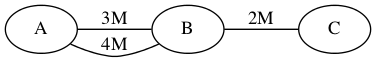
\includegraphics[width=1.3in]{3-nodes-example}
\vspace{-0.15in}
\caption{An example of the OPRE, where the traffic demand is $d_{ab}$.}
\label{figure_an_example_of_opre}
\end{figure}

Now, assume that links $l_1$ and $l_2$ consume the same power, and one link has to be switched off/sleep to save energy. Let us check the OPRE after pruning $l_1$ and $l_2$, respectively. If $l_1$ is pruned, $d_{ab}$ is put on link $l_2$, and the MLUR is $\frac{1}{4}d_{ab}$, so the OPRE is $\frac{1}{4}d_{ab}/\frac{1}{7}d_{ab} = 7/4 = 1.75$. If $l_2$ is pruned, $d_{ab}$ traverses link $l_1$, resulting in the MLUR of $\frac{1}{3}d_{ab}$, so the OPRE is $\frac{1}{3}d_{ab}/\frac{1}{7}d_{ab} = 7/3 = 2.33$. The results tell us that pruning link $l_1$ is more robust than pruning link $l_2$. This is consistent with the intuition that link $l_2$ has a larger capacity and is stronger against congestion.

\subsection{Problem Formulation}

Now we formally model the problem. Our objective is to minimize OPRE $P^*(r, M, G, G^*)$, where $M$ and $G$ are inputs, and routing $r$ and sub-graph $G^*$ are decision variables. The Min-OPRE problem is as follows.

\begin{center}
Minimize \quad $P^*(r, M, G, G^*)$
\end{center}

\begin{center}
s.t. (1),\ (4),\ (5)
\end{center}

\begin{center}
    $\forall a,b,i \in V$: \quad \quad \quad \quad \quad \quad \quad \quad \quad \quad \quad \quad \quad \quad \quad
    \vspace{-0.3in}
\end{center}

\begin{equation}
\label{equation_flow_for_routing_second}
    \begin{split}
    \sum_{j, s.t.(i,j) \in E}\hspace{-0.2in}f^{r'}_{ab}(i,j) - \hspace{-0.2in}\sum_{j, s.t.(j,i) \in E}\hspace{-0.2in}f^{r'}_{ab}(j,i) =
    \left\{
        \begin{array}{c}
        \ \ 1, \ i = a \\
        -1, \ i = b \\
        \ \ \ \ \ 0, \ i \neq a,b \\
        \end{array}
    \right.
    \end{split}
\end{equation}

\begin{center}
    \vspace{0.1in}
    $\forall a,b,i \in V$: \quad \quad \quad \quad \quad \quad \quad \quad \quad \quad \quad \quad \quad \quad \quad
    \vspace{-0.3in}
\end{center}

\begin{equation}
\label{equation_flow_for_routing}
    \begin{split}
    \sum_{j, s.t.(i,j) \in E^*}\hspace{-0.2in}f^r_{ab}(i,j) - \hspace{-0.3in}\sum_{j, s.t.(j,i) \in E^*}\hspace{-0.2in}f^r_{ab}(j,i) =
    \left\{
        \begin{array}{c}
        \ \ 1, \ i = a \\
        -1, \ i = b \\
        \ \ \ \ \ 0, \ i \neq a,b \\
        \end{array}
    \right.
    \end{split}
\end{equation}

\begin{center}
    \vspace{0.1in}
    $\forall a,b \in V$, $\forall i,j \in E$: \quad \quad \quad \quad \quad \quad \quad \quad \quad \quad \quad
    \vspace{-0.15in}
\end{center}

\begin{equation}
\label{inequation_traffic_fraction}
    0 \leq f^r_{ab}(i,j),f^{r'}_{ab}(i,j) \leq 1
\end{equation}

\begin{equation}
\label{inequation_power_threshold}
    \sum_{l \in E^*} p(l) / \sum_{l \in E} p(l) \leq 1 - \theta
\end{equation}

Constraints (\ref{equation_U_rmG}), (\ref{equation_P_rmGG}), and (\ref{equation_P_rMGG}) follow our definition of the OPRE. Eq. (\ref{equation_flow_for_routing_second}) means that the optimal routing $r'$ in $G$ must be a valid routing, i.e. with routing consistency. Specifically, for the source/destination node, all traffic must be routed/received; and for an intermediate node, the traffic flowing out must equal the traffic flowing in. Similarly, Eq. (\ref{equation_flow_for_routing}) means that the robust routing $r$ in $G^*$ must be a valid routing. Ineq. (\ref{inequation_traffic_fraction}) means that the range of $f^r_{ab}(i,j)$ and $f^{r'}_{ab}(i,j)$ is from 0 to 1. Ineq. (\ref{inequation_power_threshold}) means that the power consumption of links in $G^*$ must be less than a given threshold. In Ineq. (\ref{inequation_power_threshold}), $\theta$ denotes the power saving ratio we must achieve by using $G^*$. Here, we use $p(l)$ to denote the power consumption of link $l$, which is mainly drawn by the line cards at the two ends of the link. Note that $p(l)$ is independent of the traffic volume, and this assumption is based on the fact that in current stage, the power of a line card changes little with the traffic volume \cite{PowerAware08Infocom}.

Note that if $G^* = G$ satisfy the energy constraint Ineq. (\ref{inequation_power_threshold}) and $M$ is the set of all TMs, the Min-OPRE problem reduces to the demand-oblivious routing problem, and can be transformed into a linear program and solved in polynomial time \cite{networking:oblivious}. However, we must find the optimal $G^*$ to achieve the required power saving ratio in other cases, and Min-OPRE is an MILP and is NP-hard in general.

Also note that we put the power saving in the constraint of our problem, instead of the objective function. In such a way, we can balance the trade off between energy conservation and the OPRE, by setting different values of power saving ratio $\theta$. We can even achieve the maximum power saving ratio by a binary search on $\theta$.

\section{Upper Bounds of the Minimum OPRE}
\label{upper_bounds_of_the_minimum_opre}

In this section, we analyze the upper bounds of the minimum OPRE. We are interested in two extreme types of networks, i.e., cycles and cliques, because general networks can be seen as intermediate cases between them. We will present the upper bounds with small and large values of $\theta$. We find that, though the minimum OPR of cycles and cliques is similar and bounded by 2 \cite{networking:oblivious}, the minimum OPRE is much more different and has a larger upper bound with a larger $\theta$. These theoretical results tell us that the robust energy efficient routing exists, and tell us how close a robust routing can get to the optimal routing.

\begin{lemma}
$\min P^*(r, M, G, G^*) \geq \min P^*(r, M, G)$ if $G^* \subseteq G$, where the equation holds if $G^* = G$.
\end{lemma}
\begin{proof}
We assume exist a $G^*$, s.t. min $P^*(r,M,G,G^*)$ $<$ min $P^*(r, M, G)$. Becuase $G^*$ is the subset of $G$, we directly
use the robust routing of $G^*$ to $G$, then $P^*(r, M, G)$ will equal to $P^*(r,M,G,G^*)$, and arise contradiction.
Particularly, when $G^* = G$, $G^*$ is the subset of $G$, and $G$ is the subset of $G^*$, so there is both
min $P^*(r,M,G,G^*)$ $\geq$ min $P^*(r, M, G)$ and $P^*(r, M ,G)$ $\geq$ $P^*(r, M, G, G^*)$, so they are equal to each other
when $G^*$ = $G$. This ends our proof.
\end{proof}

\begin{theorem}
The minimum OPRE of $C_n$ (the cycle on $n$ vertices with unit capacity links) and $K_n$ (the complete graph on $n$ vertices with unit capacity links) is $2-2/n$ if $\theta = 0$.
\end{theorem}
\begin{proof}
According to Lemma 1, the minimum OPRE of $C_n$ is the minimum OPR, i.e., $\min P^*(r, M, C_n)$, when $\theta = 0$. Similarly, the minimum OPRE of $K_n$ is $\min P^*(r, M, K_n)$ when $\theta = 0$. On the other hand, we know from \cite{networking:oblivious} that the minimum OPR of $C_n$ is $2-2/n$, and the minimum OPR of $K_n$ is also $2-2/n$. This ends our proof.
\end{proof}

Theorem 2 shows the minimum OPRE when $\theta$ equals 0 and all link capacities are the same. In a more general case when there are different link capacities, we have

\begin{theorem}
The upper bound of the minimum OPRE for a cycle/complete graph on $n$ nodes is $1 + \frac{\max cap_{ij}}{\min cap_{ij}}$ if $\theta = 0$.
\end{theorem}
\begin{proof}
See Appendix A.
\end{proof}

Theorem 3 tells us that the minimum OPRE is related to the link capacity difference in the network. The above results are for $\theta = 0$. Now let us see the results for a large $\theta$. Since there is not much difference between the power consumptions for links with different capacities \cite{networking:greenfrr}, we consider the spanning trees of a graph, which can achieve a near-optimal $\theta$. We have
\begin{theorem}
Let $G^*$ be a spanning tree of a cycle on $n$ nodes, and then the upper bound of the OPRE is $1 + \frac{\max cap_{ij}}{\min cap_{ij}}$.
\end{theorem}
\begin{proof}
See Appendix B.
\end{proof}
\begin{theorem}
Let $G^*$ be a spanning tree of a complete graph on $n$ nodes, and then the upper bound of the OPRE is $\frac{n^2}{2} \frac{\max cap_{ij}}{\min cap_{ij}}$.
\end{theorem}
\begin{proof}
See Appendix C.
\end{proof}

Theorem 4 and Theorem 5 present a large gap between the OPRE upper bounds in the two types of networks, because when $G^*$ is a spanning tree, more links are pruned in the complete graph. This implies that in order to achieve more energy conservation, the OPRE may become larger quickly, and the routing becomes less robust, in the worst case. However, we can still develop effective algorithms to achieve a small OPRE and save energy in general cases, i.e., in real-world networks which have much less link densities than a complete graph.


\section{Robust Energy-Aware Routing Algorithms}
\label{robust_energy_aware_routing_algorithms}

In this section, we present our REAR approach to solve the Min-OPRE problem. We first develop the robust link pruning (RLP) algorithm. RLP selects sleeping links that we will prune from the topology, to achieve the required power saving ratio and potentially reduce the OPRE. Then, we develop the robust routing adjustment (RRA) algorithm. RRA adjusts the demand-oblivious routing that has the minimum OPR, to detour the traffic around the sleeping links.

\subsection{Algorithm RLP}

Several heuristics have been proposed to select sleeping links without the knowledge of a specific TM, with various considerations \cite{networking:car}\cite{networking:dmp}\cite{networking:grida}\cite{ESACON11InfocomWs}. However, we need a algorithm that can potentially minimize the OPRE. To this end, we first find the demand-oblivious routing that minimizes the OPR, using the linear programming approach in \cite{networking:oblivious}. Bases on the routing, we define the extended robust link utilization (ERLU), to evaluate the contribution of a link to the OPRE.

Intuitively, a link is less preferred to be pruned if there are more flows traversing the link. Though we are not aware of the TM, the traffic volume is likely to fluctuate largely if there are many flows. This means that if we prune this link, these flows have to be carried by other links in the network, and the OPRE may increase largely. On the other hand, a link is less preferred to be pruned if the link has a less capacity. This is because in the optimal demand-oblivious routing where the OPR is minimized, such a link is not likely to be heavy-loaded, and we should keep the link to maintain the robustness. Formally, let $r_0$ be the optimal demand-oblivious routing, and $u^e_{ij}$ be the ERLU of link $(i, j)$, we have
\begin{equation}
\label{equation_u_eijr}
	u^e_{ij}(r_0) = \frac {\sum_{a,b}f^{r_0}_{ab}(i,j)} {cap_{ij}}
\end{equation}

With the ERLU, we iteratively select the link with the smallest ERLU as the sleeping link. If the topology after pruning the selected link is not connected, we pass the link and continue to search. We stop the process once we have sufficient sleeping links to achieve the required power saving ratio. We develop the RLP algorithm.

\begin{table}[!th]
\begin{tabular}{ll}
\hline
\textbf{Algorithm RLP()}\\
\hline
$\:\:$\textbf{Input:} $G(V, E)$, $\theta$;\\
$\:\:$\textbf{Output:} the set of sleeping links $S$;\\
$\:\:$1:\ $r_0 \leftarrow$ the optimal demand-oblivious routing \cite{networking:oblivious} on $G$;\\
$\:\:$2:\ \textbf{for} each link $l$ in E\\
$\:\:$3:\quad\ compute ERLU $u^e_l(r_0)$, using Eq. (\ref{equation_u_eijr});\\
$\:\:$4:\ $S \leftarrow \emptyset$; $goon \leftarrow \textrm{true}$;\\
$\:\:$5:\ \textbf{while} {$goon$}\\
$\:\:$6:\quad\ $goon \leftarrow \textrm{false}$;\\
$\:\:$7:\quad\ \textbf{for} {each link $l$ in $E-S$ with increasing order based on $u^e_l(r_0)$}\\
$\:\:$8:\quad\ \quad\ $G^* \leftarrow (V, E^* = E-S-\{l\})$;\\
$\:\:$9:\quad\ \quad\ \textbf{if} {$G^*$ is connected and $\sum_{l' \in E^*} p(l') / \sum_{l' \in E} p(l') > 1 - \theta$}\\
$\:\:$10:\quad\ \quad\ \quad\ $S \leftarrow S \cup \{l\}$;\\
$\:\:$11:\quad\ \quad\ \quad\ $goon \leftarrow \textrm{true}$;\\
$\:\:$12:\quad\ \quad\ \quad\ \textbf{break};\\
$\:\:$13:\ \textbf{return} $S$;\\
\hline
\end{tabular}
\end{table}

The inputs of RLP include graph $G(V, E)$ and required power saving ratio $\theta$, and the output is the sleeping link set $S$. The ERLU of each link is computed in Steps 1 to 3. $S$ is initialized to be empty (Step 4). In each iteration of the outer loop (Steps 5 to 12), a feasible sleeping link is selected (Steps 7 to 12). If a feasible sleeping link is found and the power saving ratio is not achieved yet (Step 9), the selected link is added into set $S$ (Step 10), binary variable $goon$ will be true (Step 11), and the process continues (Step 12). Or else, binary variable $goon$ will remain false (Step 6), and the algorithm ends. The computation complexity of the RLP algorithm is $O(LP + |E||V|^2 + (|E|-|V|)|V||E|\log|E|)$ in the worst case, where $O(LP)$ is for solving the linear programming in \cite{networking:oblivious}, $O(|E||V|^2)$ is for computing the ERLU, $O(|E|-|V|)$ is the maximum number of sleeping links, and $O(|V||E|\log|E|)$ is for the connectivity check and the sleeping link search.

\subsection{Algorithm RRA}

After pruning the links, we get graph $G^*$ (if exists) that satisfies the energy conservation requirement. Now we should compute the robust routing that minimizes the OPRE. Note that we cannot simply apply the algorithm in \cite{networking:oblivious} on $G^*$, because the algorithm minimizes OPR but not OPRE. We observe that the optimal demand-oblivious routing $r_0$ minimizes the OPR in $G$, and minimizes OPRE when $G^* = G$ according to Theorem 2. Thus, to obtain a robust routing in $G^*$, we take a heuristic that adjusts routing $r_0$ to detour the traffic around the sleeping links in $G^*$.

Note that there may be multiple paths in $r_0$ between a source-destination pair. We first decompose the paths by a standard procedure given in \cite{networkflow93book}. Formally, let $p^h_{ab}$ denote the $h$-th path between nodes $a$ and $b$, and $t^h_{ab}$ be the fraction of the traffic that is routed on $p^h_{ab}$. For each $p^h_{ab}$ that traverses a sleeping link, we must find some detour paths to absorb $t^h_{ab}$. Such detour paths should not increase the OPRE too much. Recall that ERLU $u^e_{ij}(r)$ reflects the link utilization ratio without the knowledge of the TM, under routing $r$. Thus, we prefer a path whose maximum $u^e_{ij}(r)$ is small. On the other hand, the detour paths should not be too long, in order to limit the path stretch. To this end, we use YEN's algorithm \cite{networking:yens} to compute the $k$-th shortest path in graph $G^*$. We develop Algorithm RRA.

\begin{table}[!th]
\begin{tabular}{ll}
\hline
\textbf{Algorithm RRA()}\\
\hline
$\:\:$\textbf{Input:} $G(V,E)$, sleeping link set $S$,\\
$\quad\quad\ \ \ $ optimal demand-oblivious routing $r_0$, $N$;\\
$\:\:$\textbf{Output:} robust energy-aware routing $r$;\\
$\:\:$\ 1:\ $G^* \leftarrow G(V, E-S)$; $r \leftarrow r_0$;\\
$\:\:$\ 2:\ \textbf{for} {each link $l$ in $S$}\\
$\:\:$\ 3:\quad\ \textbf{for} {each $s, d \in V$}\\
$\:\:$\ 4:\quad\ \quad\ $t \leftarrow f^r_{sd}(l)$;\\
$\:\:$\ 5:\quad\ \quad\ $paths \leftarrow$ the extracted paths for $s, d$;\\
$\:\:$\ 6:\quad\ \quad\ \textbf{for} {each path $p^h_{sd} \in paths$}\\
$\:\:$\ 7:\quad\ \quad\ \quad\ \textbf{if} {$l \in path$}\\
$\:\:$\ 8:\quad\ \quad\ \quad\ \quad\ $paths$.remove($p^h_{sd}$); \\
$\:\:$\ 9:\quad\ \quad\ $yen\_paths \leftarrow$ yens\_algorithm($G^*$, $s$, $d$);\\
$\:\:$10:\quad\ \quad\ \textbf{for} {$counter = 1$ to $N$}\\
$\:\:$11:\quad\ \quad\ \quad\ compute $u^e_{ij}(r)$;\\
$\:\:$12:\quad\ \quad\ \quad\ $p \leftarrow$ the path in $yen\_paths$ with the min. $\max_{ij} u^e_{ij}(r)$;\\
$\:\:$13:\quad\ \quad\ \quad\ $p.fraction = t / N$;\\
$\:\:$14:\quad\ \quad\ \quad\ $paths$.add($p$);\\
$\:\:$15:\quad\ \quad\ $r \leftarrow paths$.merge();\\
$\:\:$16:\ \textbf{return} $r$;\\
\hline
\end{tabular}
\end{table}

The inputs of RRA include graph $G(V,E)$, sleeping link set $S$, optimal demand-oblivious routing $r_0$ in $G$, and $N$ which will be used latter. The output is the robust energy efficient routing $r$. $G^*$ and $r$ are initialized in Step 1. The main loop from Step 2 to Step 14 finds the detour paths for each sleeping link in $S$, and for each source-destination pair. The traffic fraction that should be detoured is denoted by $t$ (Step 4), and the original paths are extracted and removed from routing $r$ (Steps 5 to 8). Then, the $k$-th shortest paths are computed in Step 9. The traffic fraction of $t$ is detoured by $N$ times evenly (Steps 10 to 14), and the detour path with the minimum value of the ERLU is selected (Steps 11 and 12). In Step 15, the duplicate paths are merges and new routing $r$ that does not traverse link $l$ is obtained. The computation complexity of the RRA algorithm is polynomial. We omit the detail due to the space limitation.
\ignore{
$O((|E|-|V|)|V|^2(|R||E| + K|V|(|E| + |V|\log|V|) + N(|E||V|^2 + K|E|) + |R||E|))$ in the worst case, where $O(|E|-|V|)$ is the maximum number of sleeping links, $O(|V|^2)$ is the maximum
number of OD pairs, $O(|R||E|)$ is for computing detoured traffic and remove failed paths where $O(|R|)$ is the number of input routings, $O(K|V|(|E| + |V|\log|V|))$ is for solving the
yens algorithm where $K$ is the number of shortest paths, $O(N(|E||V|^2 + K|E|))$ is for detouring traffic fraction by $N$ times, and $O(|R||E|)$ is for merging routings.}

\begin{figure*}[!t]
\centering
\subfloat{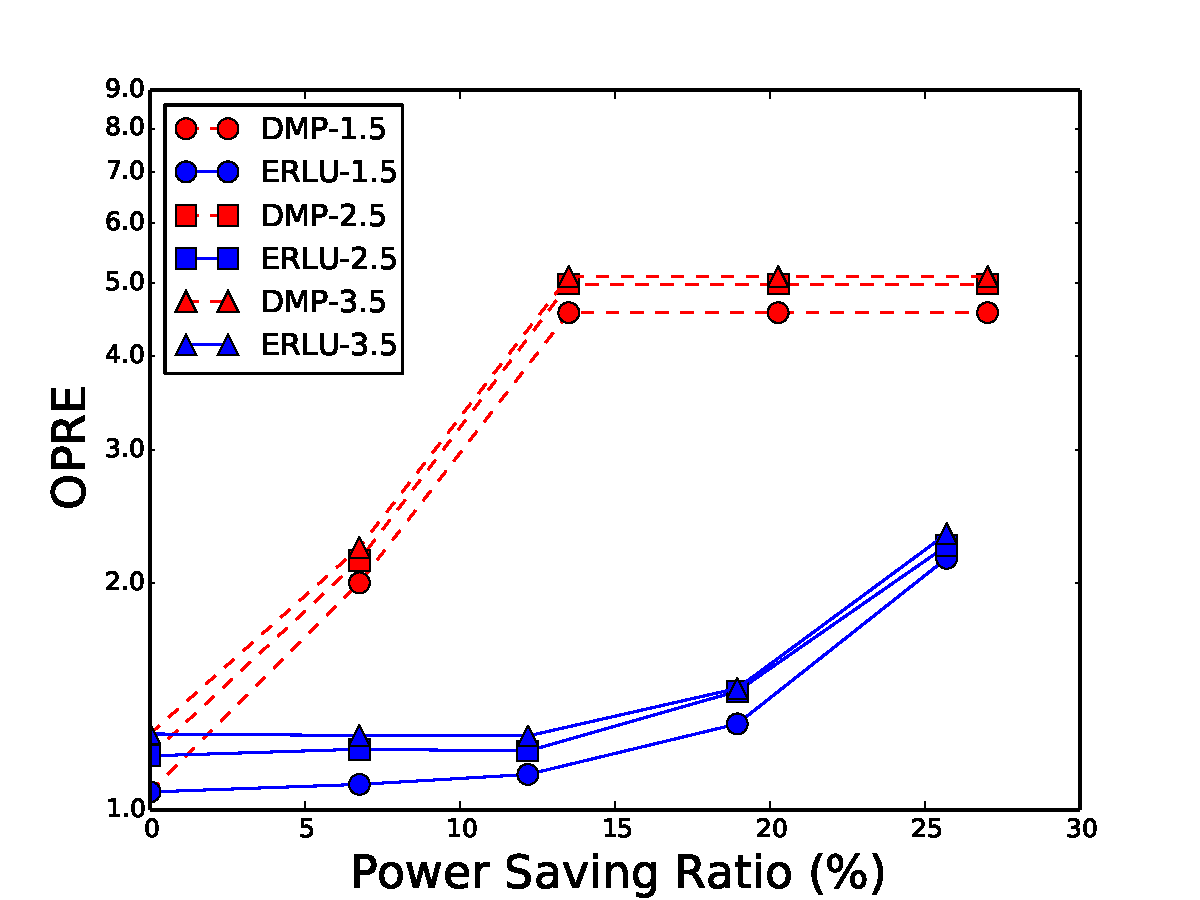
\includegraphics[width=6cm]{opr_with_power_abilene}}
\subfloat{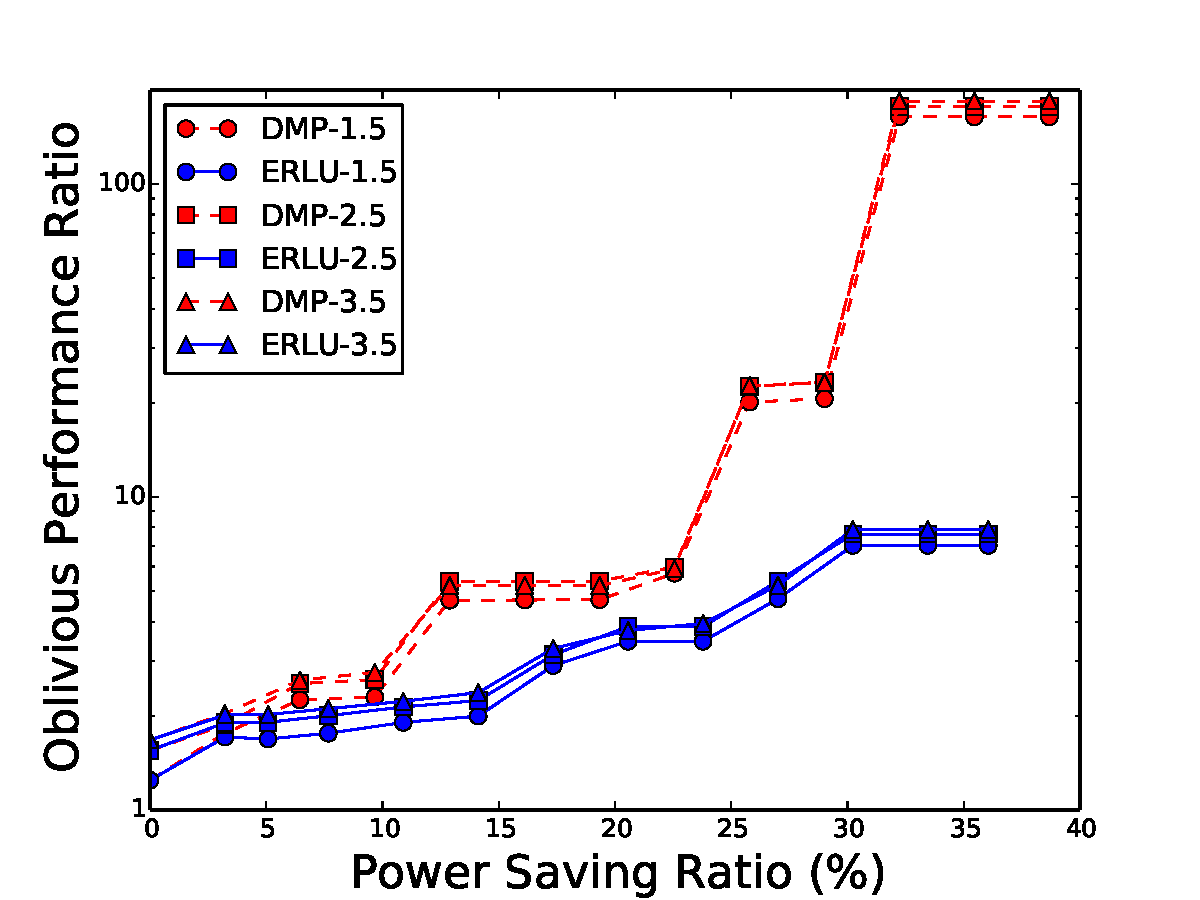
\includegraphics[width=6cm]{opr_with_power_geant}}
\subfloat{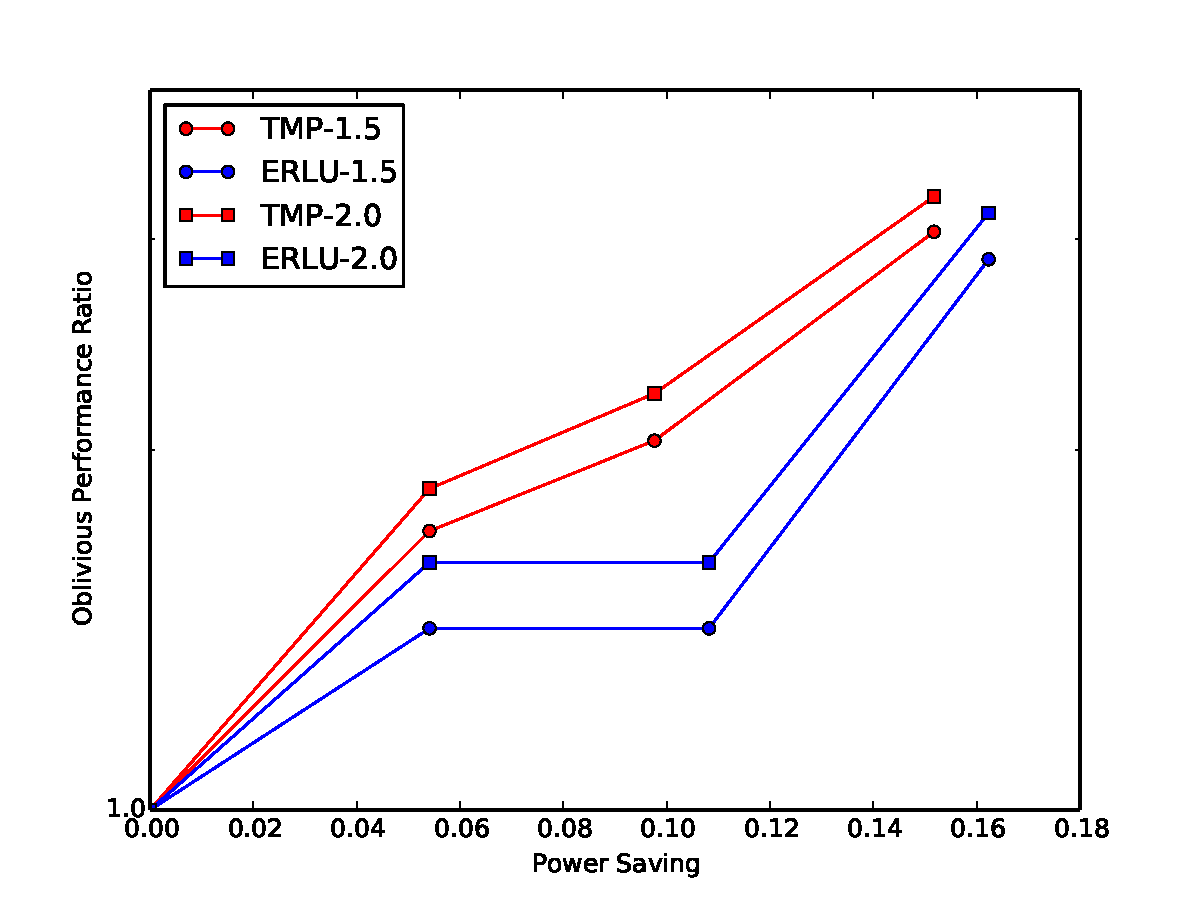
\includegraphics[width=6cm]{opr_with_power_cernet2}}
\vspace{-0.1in}
\caption{OPRE in (a) Abilene. (b) Geant. (c) CERNET2.}
\label{figure_opr_with_power}
\vspace{-0.1in}
\end{figure*}

\begin{figure*}[!t]
\centering
\subfloat{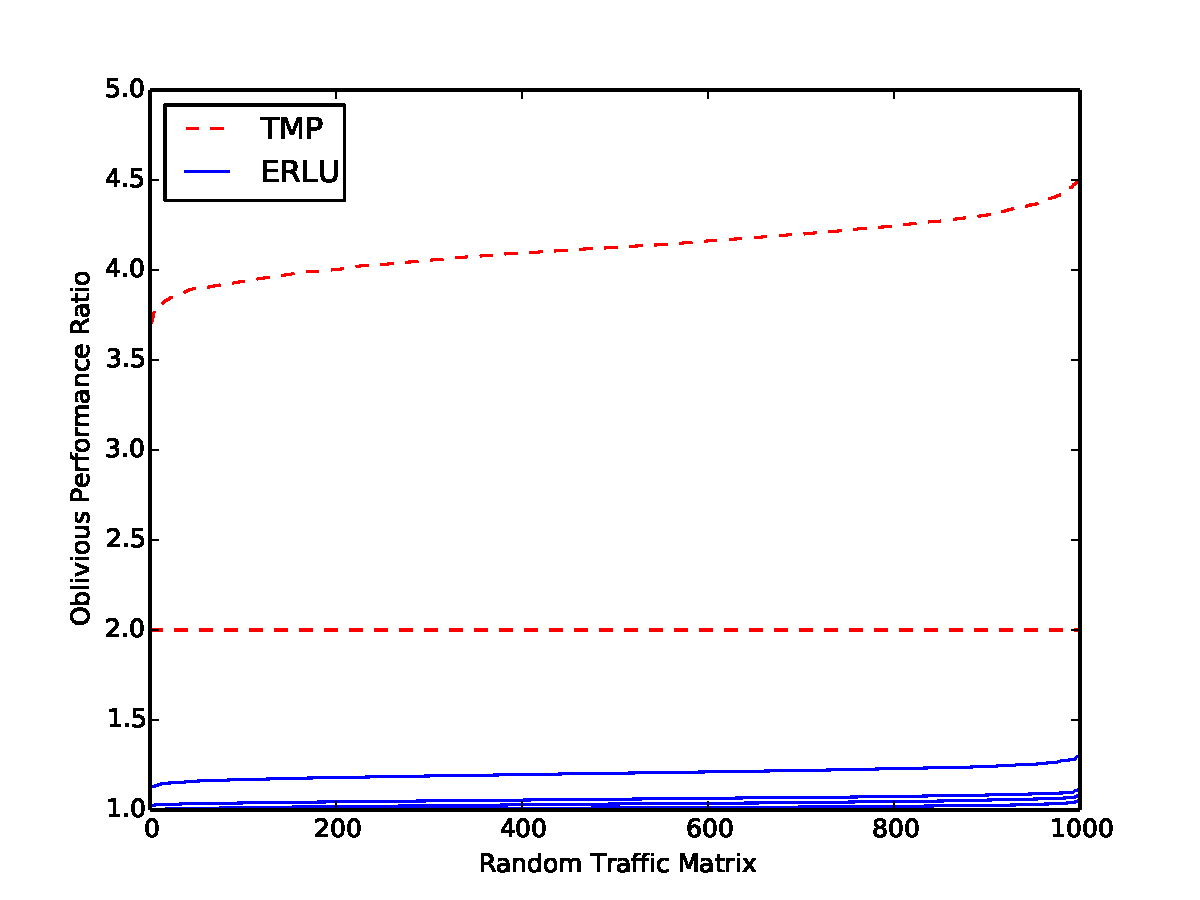
\includegraphics[width=6cm]{exp2_sort_abilene}}
\subfloat{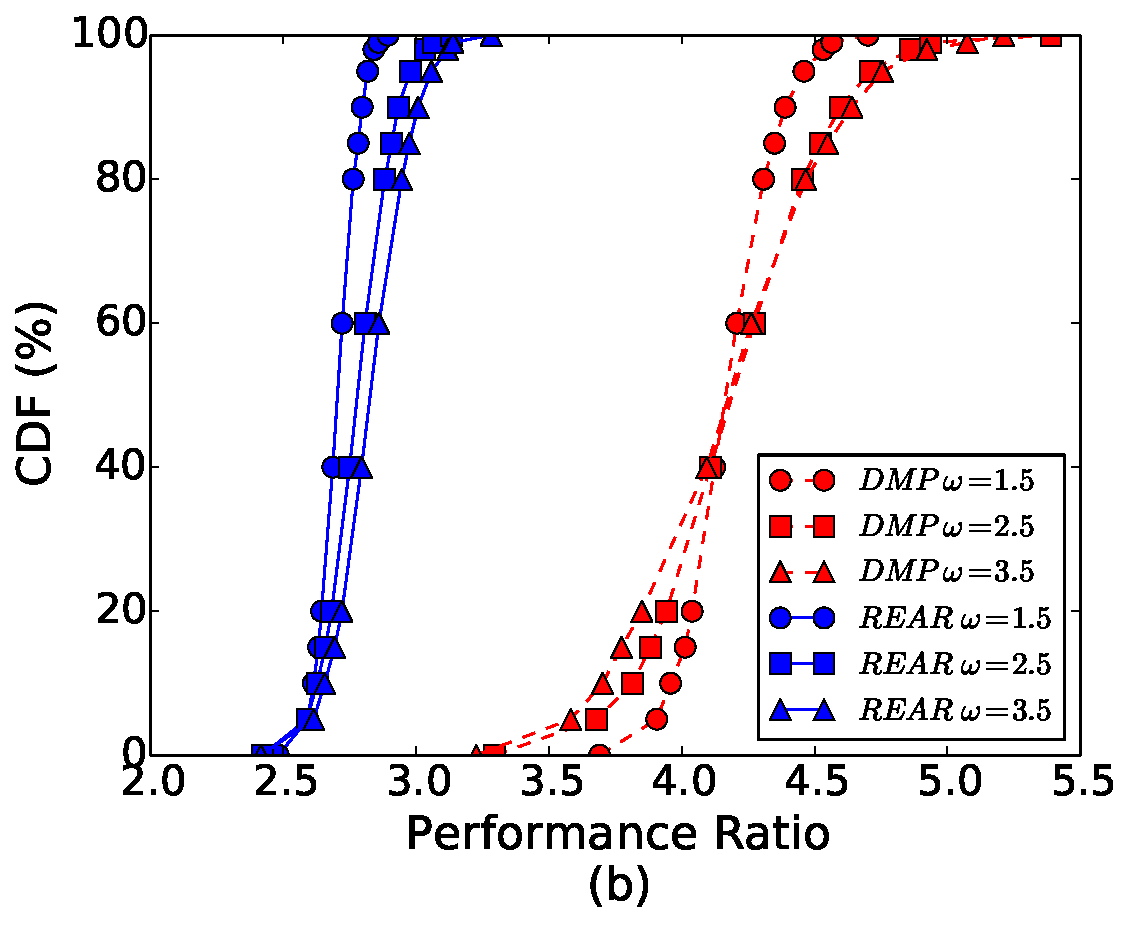
\includegraphics[width=6cm]{exp2_sort_geant}}
\subfloat{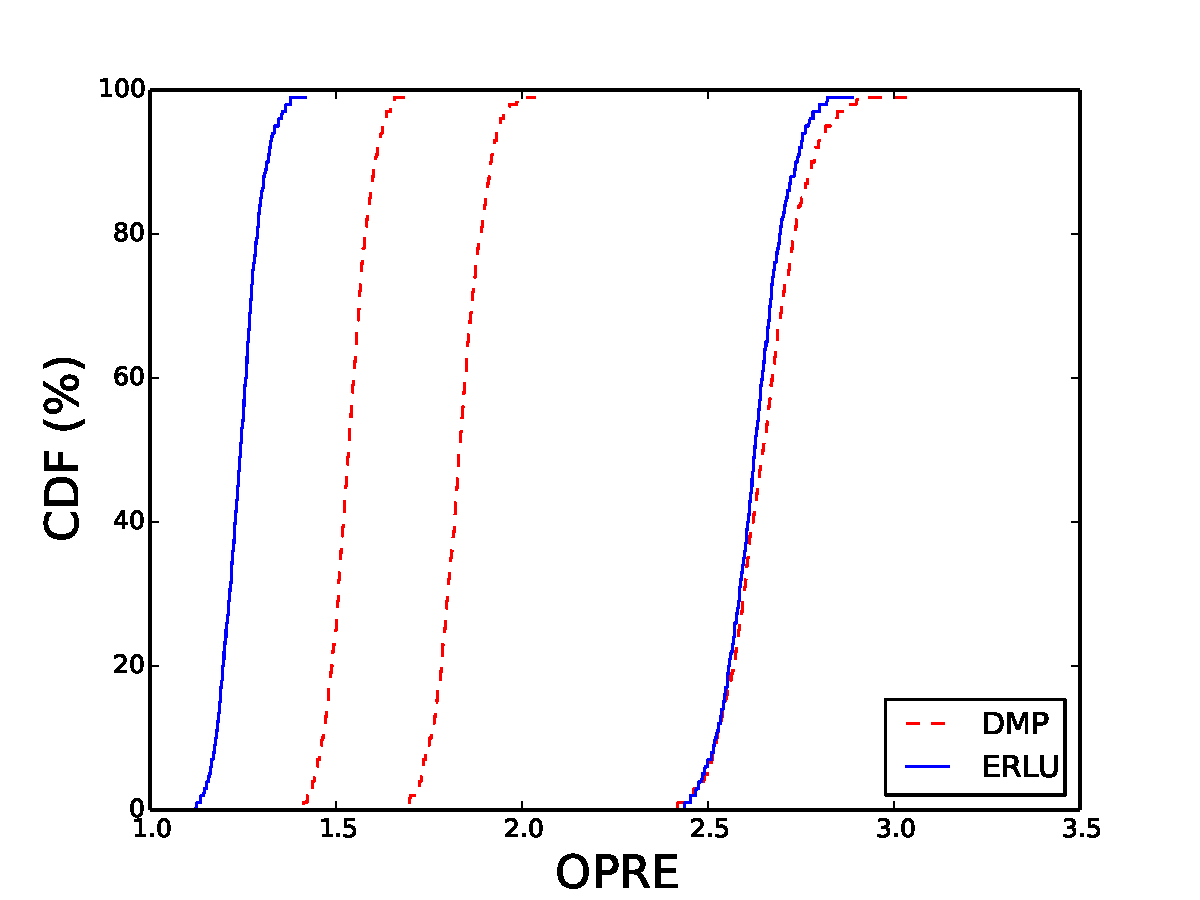
\includegraphics[width=6cm]{exp2_sort_cernet2}}
\vspace{-0.1in}
\caption{Performance ratio in (a) Abilene with 4 links pruned. (b) Geant with 6 links pruned. (c) CERNET2 with 2 links pruned.}
\label{figure_exp2_sort}
\vspace{-0.1in}
\end{figure*}


\section{Performance Evaluation}
\label{performance_evaluation}

We evaluate the REAR approach by simulations on three real-world network topologies, including Abilene \cite{networking:abilene}, Geant \cite{networking:geant}, and CERNET2 \cite{networking:cernet2}. The numbers of nodes and links of the topologies are listed in Table \ref{three_topologies}. The traffic matrices we used in our simulations are generated as follows. We first generate a baseline traffic matrix using the gravity model \cite{networking:gravity}, where the baseline traffic demand $d_{ab}$ is proportional to the total capacity of nodes $a$ and $b$. Then, the traffic demand is generated randomly in the range from $d_{ab}/\omega$ to $d_{ab}\omega$, where $\omega \geq 1$ is a margin factor used to control the fluctuation range of the traffic. We generate 1000 random TMs for each topology with each $\omega$. The power consumption of different line cards is set as constant in the simulations, as shown in Table \ref{table_line_card_power_consumption}, following \cite{networking:greente}.

\begin{table}[h]
\renewcommand{\arraystretch}{1}
\caption{Topologies}
\label{three_topologies}
\centering
\begin{tabular}{|c|c|c|c|}
\hline
\bfseries Topology & \bfseries Nodes & \bfseries Links & \bfseries Links can be Removed \\
\hline
Abilene & 12 & 15 & 4 \\
\hline
Geant & 23 & 37 & 15 \\
\hline
CERNET2 & 20 & 22 & 3 \\
\hline
\end{tabular}
\end{table}

For comparison, we simulate a recent energy efficient routing approach, namely DMP \cite{networking:dmp}, which also does not use the TMs as inputs. DMP always selects the most power-hungry links to switch into off/sleep mode, and can achieve a large power saving ratio, but does not consider routing robustness. For the approaches, we evaluate the OPRE, the power saving ratio, the distribution of the performance ratio, and the path stretch.

\begin{table}[h]
\renewcommand{\arraystretch}{1}
\caption{Line Card Power Consumption}
\label{table_line_card_power_consumption}
\centering
\begin{tabular}{|c|c|c|}
\hline
\bfseries Line-Card & \bfseries Speed(Mbps) & \bfseries Power(Watts) \\
\hline
1-Port OC3 & 155.52 & 60 \\
\hline
8-Port OC3 & 1244.16 & 100 \\
\hline
1-Port OC48 & 2488.32 & 140 \\
\hline
1-Port OC192 & 9953.28 & 174 \\
\hline
\end{tabular}
\end{table}

\begin{figure*}[!t]
\centering
\subfloat{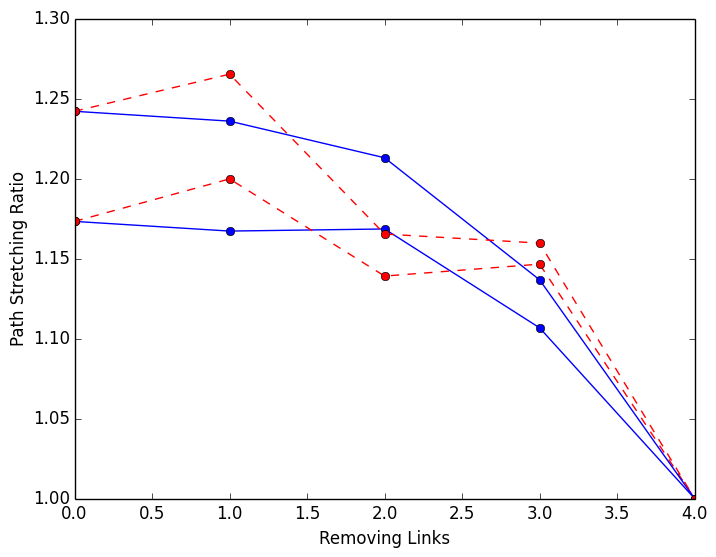
\includegraphics[width=6cm]{exp4_path_abilene}}
\subfloat{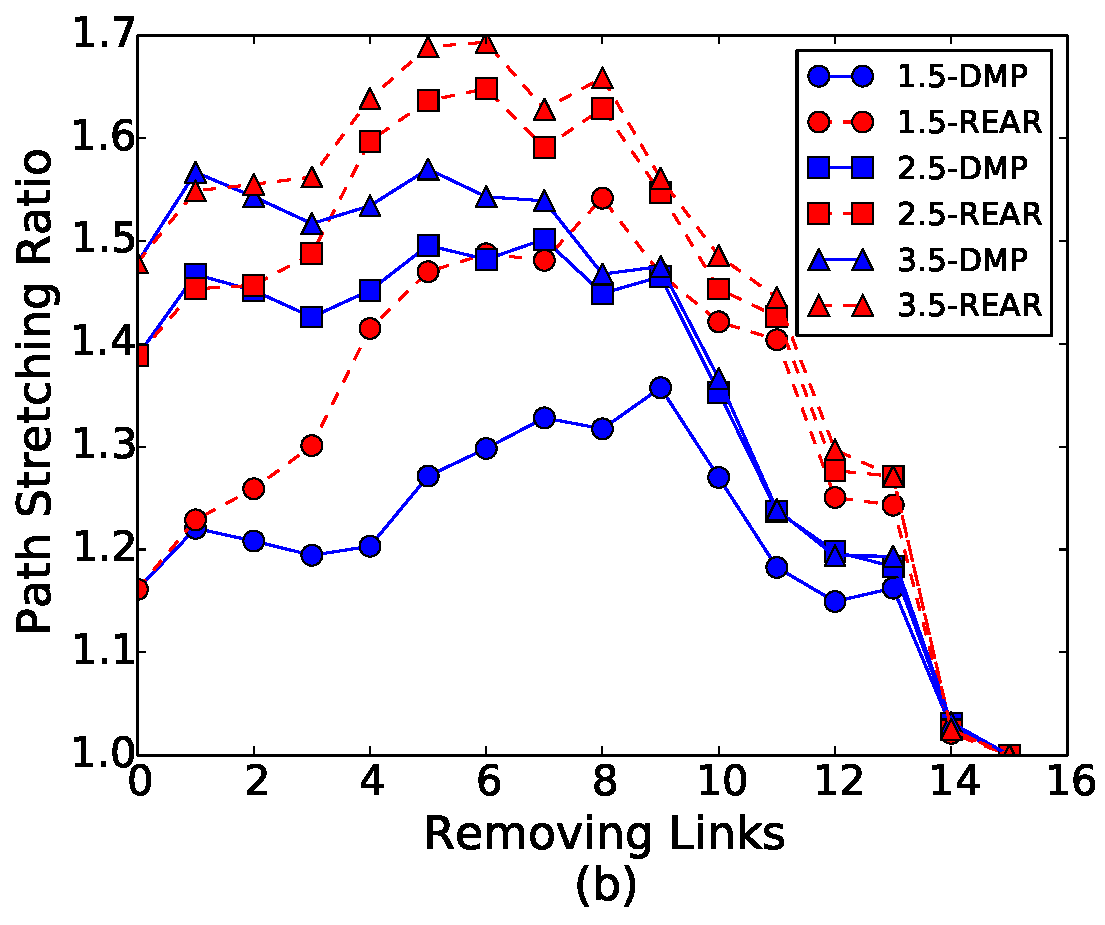
\includegraphics[width=6cm]{exp4_path_geant}}
\subfloat{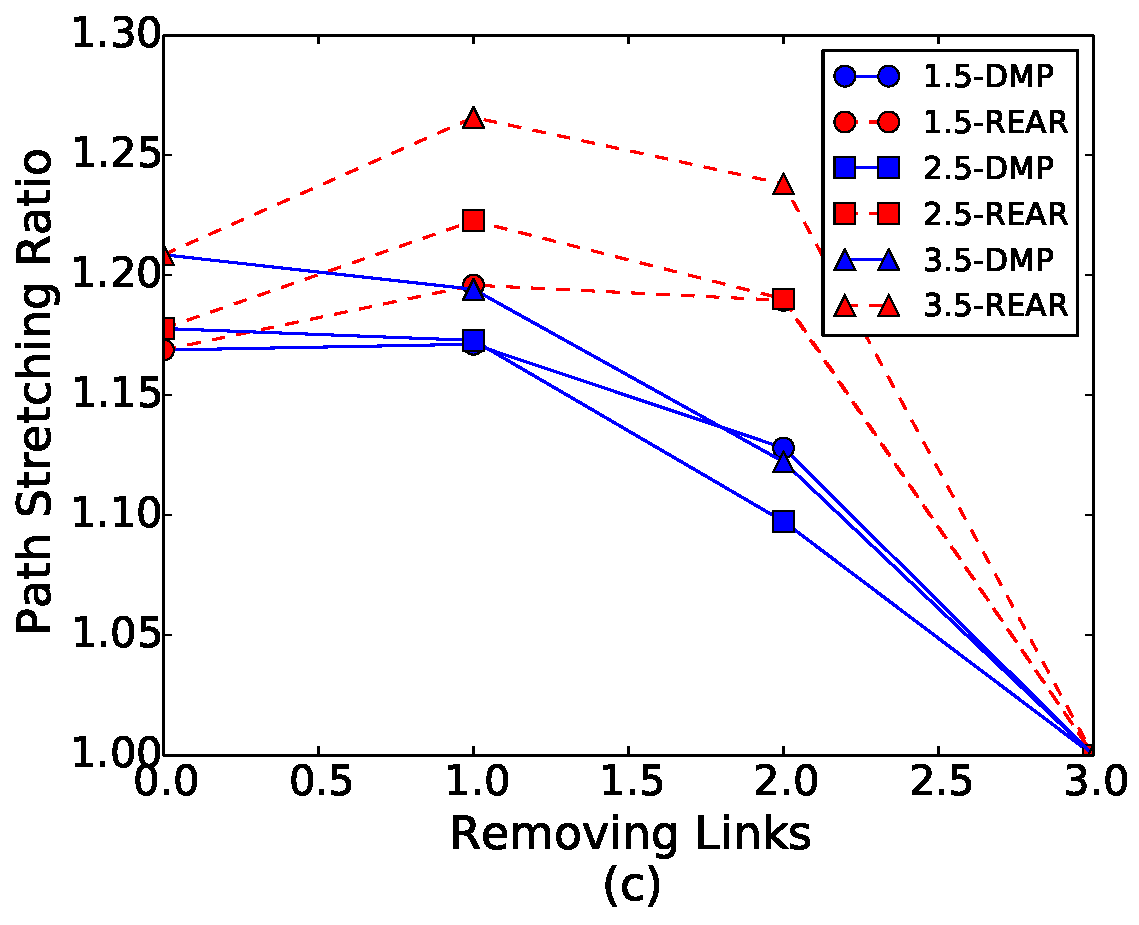
\includegraphics[width=6cm]{exp4_path_cernet2}}
\vspace{-0.1in}
\caption{Path Stretch in (a) Abilene. (b) Geant. (c) CERNET2.}
\label{figure_exp4_path}
\vspace{-0.1in}
\end{figure*}

\subsection{OPRE versus Power Saving}
Fig. \ref{figure_opr_with_power} (a) shows the OPRE (evaluated by the maximum performance ratio under all 1000 TMs), as a function of power saving ratio $\theta$, in the Abilene topology. We see that the OPRE increases when more power is saved. This is not surprising because the routing becomes less robust when more links are switched into off/sleep mode. Our REAR has an OPRE ranging from 1.06 to 2.32, which is much less than the results of DMP. This is because REAR takes routing robustness into consideration when it prunes
links and computes routing. For instance, when $\omega = 3.5$ and 25\% power is saved, the OPRE of REAR is 2.32, while the OPRE of DMP is 5.09.
This implies that REAR is more robust against traffic uncertainty. We also see that a larger $\omega$ results in a larger OPRE, because
the traffic volume fluctuates in a wider range. For instance, when $\omega$ increases from 1.5 to 3.5, the OPRE of REAR increases about
0.17, while the OPRE of DMP increases about 0.53.

Fig. \ref{figure_opr_with_power} (b) shows the OPRE as a function of power saving ratio $\theta$ in Geant. We find that the results are similar to that in Abilene. However, the OPRE is larger in Geant than in Abilene for both REAR and DMP. One reason for this result is that Geant has a larger link density ($\frac{37}{23} = 1.61$) than Abilene ($\frac{15}{12} = 1.25$). Another reason is that the link capacity difference is large in Geant. The maximum link capacity is 9920 Mbps while the minimum link capacity is 155 Mbps. Such results are consistent with our analysis in Section IV.

Fig. \ref{figure_opr_with_power} (c) shows the results in CERNET2. We observe that the difference between REAR and DMP is small. This is because the CERNET2 topology has a small link density, and only a small number of links can be pruned.

\subsection{Performance Ratio Distribution}
Fig. \ref{figure_exp2_sort} (a) shows the CDF of random TMs as a function of the performance ratio, in Abilene with 4 links pruned. The curves of REAR are on the left of DMP, which means that REAR has a lower performance ratio under all TMs. We observe that the performance ratio has a larger range with a larger $\omega$, but the performance ratio of REAR has a small range in total (e.g., from 1.74 to 2.32 when $\omega = 3.5$), unlike DMP (e.g., from 2.97 to 5.09 when $\omega = 3.5$). This implies that REAR is more robust.

Fig. \ref{figure_exp2_sort} (b) shows the results in Geant with 6 links pruned, and Fig. \ref{figure_exp2_sort} (c) shows the results in CERNET2 with 2 links pruned. The results are similar to that in Abilene.

\subsection{Path Stretch}

Now we evaluate the path stretch of the approaches, which reflects the end-to-end delay increment due to link pruning and robust routing. Here, path stretch is the ratio of the path length of a routing to the shortest path length, in the topology after pruning links. Note that there may be multiple paths in the robust routing for a source-destination pair. In such a case, we compute the weighted path stretch of these paths according to the traffic fraction they carry.

Fig. \ref{figure_exp4_path} (a) shows the path stretch as a function of pruned link number in Abilene. Generally, the path stretch decreases when more links are pruned, and equals 1 when 4 links are pruned. This is because the topology becomes less connected when more links are pruned, and reduces to a spanning tree when 4 links are pruned. The path stretch of REAR is less than 1.32, because we use YEN's algorithm to find the $k$-th shortest path when searching for paths to detour the traffic. We think this path stretch is small and will not induce large end-to-end delay increment. The path stretch of REAR is a little larger than that of DMP in some cases. This is because most links in Abilene has the same capacity and consumes the same power, and in such a case, DMP randomly selects sleeping links, which may result in less path stretch. We also observe that the path stretch increases with $\omega$, because the demand-oblivious routing is computed based on $\omega$, and when $\omega$ increases, the routing will use more paths to increase the robustness.

Fig. \ref{figure_exp4_path} (b) and (c) show the path stretch in Geant and CERNET2, respectively. We see that our REAR has a less path stretch than DMP. For instance, REAR has the largest path stretch of 1.35 in Geant when $\omega = 1.5$, while the result of DMP is 1.54.


\section{Conclusion and Future Work}
\label{conclusion}

In this paper, we studied energy efficient routing under uncertain traffic demands. We proposed metric OPRE, which defines the distance between a routing and the optimal routing with respect to the maximum link utilization ratio under energy conservation requirements. We modeled the problem of minimizing the OPRE and analyzed the upper bounds of the solution. Then, we developed the REAR scheme to solve the problem. We did simulations using real network topologies and showed that REAR can saving energy without knowing traffic matrices, and can achieve a smaller OPRE than existing approaches.

In the future, we plan to improve our algorithms, because solving the linear programming does not scale well to large networks. We are also interested in realizing the robust energy-aware routing in a hop-by-hop fashion, without fractional traffic and MPLS tunnels.

\begin{thebibliography}{1}

\bibitem{networking:greente}
M. Zhang, C. Yi, B. Liu, et al. ``GreenTE: Power-Aware Traffic Engineering," in Proc. of IEEE ICNP, October 2010.

\bibitem{networking:active}
S. Avallone, G. Ventre. ``Energy efficient online routing of flows with additive constraints." Computer Networks, vol. 56, 2368--2382, 2012.

\bibitem{ROD2012Networking}
M. Shen, H. Liu, K. Xu, et al. ``Routing On Demand: Toward the Energy-Aware Traffic Engineering with OSPF." in Proc. of IFIP Networking, 2012, 232--246.

\bibitem{Response11Conext} N.~Vasic, P.~Bhurat, D.~Novakovic,
    M.~Canini, S.~Shekhar, and D.~Kostic,
  ``{I}dentifying and using energy-critical paths,'' in Proc. of CoNext'11, 2011.

\bibitem{networking:car}
A. Cianfrani, V. Eramo, M. Listanti, and M. Polverini, ``An OSPF enhancement for energy saving in IP networks," in IEEE INFOCOM Workshop on Green Communications and Networking, April 2011.

\bibitem{networking:dmp}
A.P. Bianzino, L. Chiaraviglio, M. Mellia, ``Distributed algorithms for green IP networks," in: IEEE INFOCOM Workshop on Green Networking and Smart Grid, 2012

\bibitem{networking:grida}
A. P. Bianzino, L. Chiaraviglio, M. Mellia, et al. ``GRiDA: GReen Distributed Algorithm for energy-efficient IP backbone networks," Computer Networks, vol.~56, 3219-–3232, 2012.

\bibitem{networking:greenfrr}
Y. Yang, M. Xu, Q. Li. ``Towards fast rerouting-based energy efficient routing," Computer Networks, vol.~70(9), 1--15, 2014.

\bibitem{SPEED14TON}
Q. Li, M. Xu, Y. Yang, L. Gao, Y. Cui, and J. Wu. ``Safe and Practical Energy-Efficient Detour Routing in IP Networks,'' IEEE/ACM Transactions on Networking, vol.~22(6), 1925--1937, 2014.

\bibitem{ESACON11InfocomWs} F.~Cuomo, A.~Abbagnale,
    A.~Cianfrani, and M.~Polverini, ``{K}eeping the
  {C}onnectivity and {S}aving the {E}nergy in the {I}nternet,'' in \emph{IEEE INFOCOM Workshop on GCN}, April 2011.
  
\bibitem{DynamicVSOblivious11Algorithmica}
N. Goyal, N. Olver, F. B. Shepherd. ``Dynamic vs. Oblivious Routing in Network Design,'' Algorithmica, vol. 61(1), 161--173, 2011.

\bibitem{networking:minimize}
Harald R\"{a}cke. ``Minimizing congestion in general networks," In Proceedings of the 43rd IEEE Symposium on Foundations of Computer Science (FOCS), 2002. Co-Winner of Best Paper Award.

\bibitem{networking:polynomial}
Y. Azar, E. Cohen, A. Fiat, H. Kaplan, and H. R acke. ``Optimal oblivious routing in polynomial time," In Proceedings of the 35th ACM Symposium on the Theory of Computing, 2003.

\bibitem{networking:oblivious}
D. Applegate and E. Cohen, ``Making Intra-Domain Routing Robust to Changing and Uncertain Traffic Demands: Understanding Fundamental Tradeoffs," in Proceedings of ACM SIGCOMM ’03, Karlsruhe, Germany, August 2003.

\bibitem{ASimpleMethodBalancing05ICCCN}
Y. Li, J. Harms, R. Holte. ``A simple method for balancing network utilization and quality of routing,'' in Proc. of ICCCN, 2005.

\bibitem{TrafficOblivious07CommuMagazine}
M. Kodialam, T. V. Lakshman, S. Sengupta. ``Traffic-Oblivious Routing for Guaranteed Bandwidth Performance,'' IEEE Communications Magazine, vol. 45(4), 46--51, 2007.

\bibitem{ObliviousHighVariable08TON}
M. Kodialam, T. V. Lakshman, J. B. Orlin, S. Sengupta. ``Oblivious Routing of Highly Variable Traffic in Service Overlays and IP Backbones,'' IEEE/ACM Trans. on Netw., vol. 17(2), 459--472, 2008.

\bibitem{ObliviousHoseModel11TON}
M. Kodialam, T. V. Lakshman, J. B. Orlin, S. Sengupta. ``End-to-End Restorable Oblivious Routing of Hose Model Traffic," IEEE/ACM Trans. on Netw., vol. 19(4), 1223--1236, 2011.

\bibitem{networking:gravity}
M. Roughan, A. Greenberg, C. Kalmanek, M. Rumsewicz, J. Yates, and Y. Zhang. ``Experience in measuring backbone traffic variability: models, metrics, measurements, and meaning," InProceedings of the 2nd Internet Measurement Workshop. ACM, 2002.

\bibitem{PowerAware08Infocom} J.~Chabarek, J.~Sommers,
    P.~Barford, C.~Estan, D.~Tsiang, and S.~Wright,
  ``{P}ower {A}wareness in {N}etwork {D}esign and {R}outing,'' in \emph{Proc.
  of IEEE INFOCOM}, 2008, pp. 457--465.

\bibitem{networkflow93book}
R. K. Ahuja, T. L. Magnanti, J. B. Orlin. Network flows: theory, algorithms, and applications. Prentice Hall, Feb., 1993.

\bibitem{networking:yens}
Yen, Jin Y. ``Finding the k Shortest Loopless Paths in a Network," Management Science 17 (11), 1971.

\bibitem{networking:abilene}
``Abilene Core Topology," [Online], Available:\\ https://itservices.stanford.edu/service/network/internet2/abilene

\bibitem{networking:geant}
``Geant Topology," [Online], Available:\\ http://geant3.archive.geant.net/Network/NetworkTopology/pages/home.aspx

\bibitem{networking:cernet2}
``CERNET2 Topology," [Online], Available:\\ http://www.edu.cn/20060111/3170220.shtml

\end{thebibliography}

\appendices

\section{Proof of Theorem 3}
\begin{proof}
We compute the optimal routing for some arbitrary TM and forward the demands on the topologies. Let $d_l$ be the 
traffic on link $l$, and $cap_l$ be the capacity of link $l$. For circles and cliques are highly homomorphic,
without loss of generality we say the link $l_1$ is the bottleneck, i.e. the link with MLUR.


Routing can be adjusted. We image a simple situation that forward the traffic from one link to another path base
on the routing computed above. The link utilization of links on the path will increase, while accordingly the 
link utilization of adjusted link will reduce to 0. Obliviously, the adjusted routing must not be better than
the optimal robust routing, so its upper bound also is the bound of minimum OPRE. Following proof is according 
to which the adjusted link is, and which the bottleneck is after adjusting routing.

For Case \Rmnum{1}.\Rmnum{1}, the adjusted link is $l_2$, the new bottleneck still be $l_1$. Because $l_1$ is the 
bottleneck before adjusting, so we have inequation:

\begin{equation}
\label{inequation_A_1_1_1}
\frac {d_2} {cap_2} \leq \frac {d_1} {cap_1} \Longleftrightarrow \frac {d_2}{d_1} \leq \frac{cap_2}{cap_1}
\end{equation}

we compute OPRE for Case \Rmnum{1}.\Rmnum{1} combined with Ineq. (\ref{inequation_A_1_1_1}):

\begin{equation}
\label{inequation_A_1_1_result}
\frac {\frac{d_1 + d_2}{cap_1}} {\frac{d_1}{cap_1}} = 1 + \frac{d_2}{d_1} \leq 1 + \frac{cap_2}{cap_1}
\end{equation}


For Case \Rmnum{1}.\Rmnum{2}, the adjusted link also be $l_2$, but the new bottleneck may be $l_3$.
Because $l_1$ is the bottleneck before adjusting, so we have inequations:

\begin{equation}
\label{inequation_A_1_2_1}
\frac {d_3} {cap_3} \leq \frac {d_1} {cap_1} \Longleftrightarrow \frac {d_3 * cap_1}{d_1 * cap_3} \leq 1
\end{equation}

\begin{equation}
\label{inequation_A_1_2_2}
\frac {d_2} {cap_2} \leq \frac {d_1} {cap_1} \Longleftrightarrow \frac {d_2 * cap_1}{d_1} \leq cap_2
\end{equation}

We compute OPRE for Case \Rmnum{1}.\Rmnum{2} combined with Ineq. (\ref{inequation_A_1_2_1}) and Ineq. (\ref{inequation_A_1_2_2}):

\begin{equation}
\label{inequation_A_1_2_result}
\frac {\frac{d_3 + d_2}{cap_3}} {\frac{d_1}{cap_1}} =
\frac {d_3 * cap_1}{d_1 * cap_3} + \frac {d_2 * cap_1}{d_1 * cap_3} \leq 1 + \frac{cap_2}{cap_3}
\end{equation}


For Case \Rmnum{2}, the adjusted link is $l_1$, namely the old bottleneck link, the new bottleneck
maybe $l_3$. Computing the OPRE combined with Ineq. (\ref{inequation_A_1_2_1}):

\begin{equation}
\label{inequation_A_2_result}
\frac {\frac{d_3 + d_1}{cap_3}} {\frac{d_1}{cap_1a}} =
\frac {d_3 * cap_1}{d_1 * cap_3} + \frac{cap_1}{cap_3} \leq 1 + \frac{cap_1}{cap_3}
\end{equation}


To sum up, we have inequation from Ineq. (\ref{inequation_A_1_1_result}), Ineq. (\ref{inequation_A_1_2_result}) and Ineq. (\ref{inequation_A_2_result}):

\begin{equation}
\label{inequation_A_result}
1 + \max \{\frac{cap_2}{cap_1}, \frac{cap_2}{cap_3}, \frac{cap_1}{cap_3} \} \leq 1 + \frac{\max_{l \in E} cap_{l}}{\min_{l \in E} cap_{l}}
\end{equation}

\end{proof}

\section{Proof of Theorem 4}
\begin{proof}
The spanning tree of circle is the topology which lose one link. 
We regard this link as the adjusted link mentioned in Appendix. A. The complete proof is almost the same with Appendix. A.
\end{proof}

\section{Proof of Theorem 5}
\begin{proof}
Suppose clique has $n$ nodes, every link in the spanning tree will split the tree to two components. 
Let $l_3$ be the bottleneck in the spanning tree, Let $S$, $D$ be the node sets of two components, and every flow 
between $S$ and $D$ always trace on $l_3$. Without loss of generality, we say $l_1$ is the bottleneck link for the 
optimal routing on the original clique.

Because the $l_1$ is the bottleneck link, we have:

\begin{equation}
\label{ineqaution_C_1}
    \frac{d_l}{cap_l} \leq \frac{dem_1}{cap_1} \Longleftrightarrow \frac{d_l * cap_1}{d_1} \leq cap_l,  \forall l \in (S,D)
\end{equation}


The $l_3$ is the bottleneck finally, we have OPRE combined with Ineq. (\ref{ineqaution_C_1}):

\begin{equation}
\label{ineqaution_C_2}
    \frac{\frac{\sum_{l \in (S,D)} d_l}{cap_3}}{\frac{d_1}{cap_1}} = \frac{cap_1}{cap_3} \sum_{l \in (S,D)} \frac{d_l}{d_1}
     \leq \sum_{l \in (S,D)} \frac{cap_l}{cap_3}
\end{equation}

And we know that, the amount of $l$ must less than $\frac{n^2}{2}$ (equal to $\frac{n^2}{2}$ if $|S| == |D| == \frac{n}{2}$), 
so OPRE must lower than:

\begin{equation}
\label{ineqaution_C_result}
    \sum_{l \in (S,D)} \frac{cap_l}{cap_3} \leq \frac{n^2}{2} \frac{\max_{l \in (S,D)} cap_l}{\min_{l \in (S,D)} cap_l}
\end{equation}

\end{proof}

% that's all folks
\end{document}



























